\documentclass{article}

\usepackage{booktabs,soul,tabu,pdfpages}		
\usepackage{enumerate}
\usepackage{tabularx}
\newcolumntype{C}{>{\centering\arraybackslash}X}
\newcolumntype{K}{>{\centering\arraybackslash}X}
%\usepackage{bm}
\usepackage[english]{babel}
\usepackage{lmodern}
\usepackage[utf8]{inputenc}
\usepackage[T1]{fontenc}
\usepackage{graphicx}
\usepackage[round]{natbib}
\usepackage{hyperref}					
\usepackage{booktabs,tabularx}
\usepackage{color,enumerate}
\usepackage{caption}
\usepackage{amsmath,amstext,amssymb} 
\usepackage{tabu,booktabs,color,pdfpages}



\title{A \LaTeX{} Template\thanks{Some comment}}
\author{Your Name  \\
	Contact (email) \\
	\and 
	The Other Dude \\
	Contact (email) \\
}
\date{\today}

\begin{document}
	\maketitle
	
\begin{abstract}
	This Template guides how to write a good course description.\footnote{More information can be found here: \url{www.chronicle.com/article/how-to-create-a-syllabus/} and here: \url{https://teaching.utoronto.ca/teaching-support/course-design/developing-a-syllabus/}}
%	Overall, I would say that the course description should have a maximum length of three pages.	
\end{abstract}
	
\subsubsection*{Course Description}
	Course descriptions should:
\begin{itemize}
	\item Be student-centered, rather than teacher-centered or course-centered
	\item Use brief, outcomes-based, descriptive phrases that begin with an imperative or active verb (e.g., design, create, plan, analyze)
	\item Be clear, concise, and easy to understand (< 100 words)
	\item Detail significant learning experiences and benefits students can expect
	\item Align with the outcomes identified in the rest of the course outline
\end{itemize}	
	Course descriptions should avoid:
\begin{itemize}
	\item Obvious, redundant, or repetitive language (such as “this course will…” or “students should expect to…”)
	\item Marketing language (such as ``Concept X is a critical part of success in Industry Y'' or ``Course A will change the way you think about everything'')
\end{itemize}
	
\subsubsection*{Prerequisites}

\subsubsection*{Course Learning Outcomes}

Course Learning Outcomes (CLO) articulate to students, faculty, and others what students will achieve in the course.
A learning outcome  is a measurable, observable, and specific statement that clearly indicates what a student should know and be able to do as a result of learning.

Well-written learning outcomes involve the following parts (also see \autoref{fig:cl}):
\begin{itemize}
\item Action verb
\item Subject content 
\item Level of achievement 
\item Condition of performance (if applicable)
\end{itemize}

\noindent \textbf{\textit{A list may look like this:}}
\begin{enumerate}[CLO 1]
	\item bla 
	\item bla bla
\end{enumerate} 


\begin{figure}
	\centering
	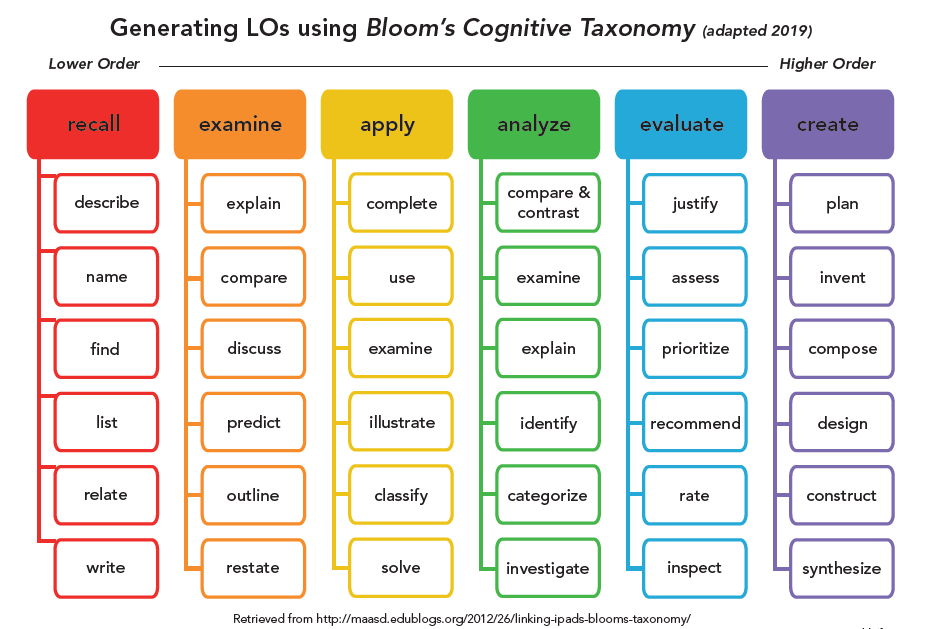
\includegraphics[width=0.85\linewidth]{cl}
	\caption{Select an Action Verb Using Bloom’s Taxonomy:}\label{fig:cl}
	
\tiny	Source: \url{https://www.mohawkcollege.ca/sites/default/files/CTL/Blooms\%20Taxonomy.png}
\end{figure}

A general hint for writing titles is: use a capitalization styles (\url{https://capitalizemytitle.com/}).

\subsubsection*{Course Materials}

\subsubsection*{About the Lecturer}



\section{\LaTeX Stuff}

Tutorials how to install \LaTeX{} on your PC can be found online, see e.g. \url{https://www.latex-project.org/get/}. I personally use TeXstudio\footnote{\url{www.texstudio.org}}  which is a cross-platform open-source \LaTeX\ editor. Its features include an interactive spelling checker, code folding, and syntax highlighting. It does not provide \LaTeX\ itself -- the user must install \LaTeX\ first.

This template is written for the article class, which is an important documentclass. For more specialized purposes there are other \textbf{documentclasses} available like \textit{book} see page \pageref{book}, \textit{report} or \textit{letter} which are 
	described in Section \ref{documentclasses}. 
	
\subsection{Documentclasses}\label{documentclasses}
In \LaTeX\ different \textit{documentclasses} exist:	
	\begin{enumerate}
		\item article
		\item book 
		\item report 
		\item letter 
	\end{enumerate}
	
	\begin{description}
		\item[article\label{article}]{Article is \ldots}
		\item[book\label{book}]{The book class \ldots}
		\item[report\label{report}]{Report gives you \ldots}
		\item[letter\label{letter}]{If you want to write a letter.}
	\end{description}

You can also build list by your own, e.g.:
\begin{enumerate}[a)]
	\item bla bla
	\item bla bla bla
\end{enumerate}

You can create tables like \autoref{tab:eins} or figures like Figure \ref{fig:latexcover} in a floating environment. Here are some guidelines to make your tables look good  \url{https://people.inf.ethz.ch/markusp/teaching/guides/guide-tables.pdf}	

\begin{table}
	\begin{center}
		\caption{This is a Table}\label{tab:eins}
		\begin{tabular}{ c c c }\toprule
			header a & header b & header c \\\midrule
			a & b & c \\
			a & b & c \\\bottomrule
		\end{tabular}\\[.5em]
\tiny Source: I did it.
	\end{center}
\end{table}

\begin{figure}
	\centering
	
\includegraphics[width=0.4\linewidth]{LaTeX_cover}
	\caption{This is a Figure}\label{fig:latexcover}
\end{figure}


	
	\section{How to Include Literature}\label{conclusions}
It is easy to include references to literature in \LaTeX.

With the command \texttt{$\backslash$nocite\{*\}} you can include all the references of a .lit-database. I do that here. However, usually you include only the literature that is mentioned in the text to your reference list. \LaTeX\ will do most of the work for you. You just need to enter the requried informations about a book or an article in the .bib database.\footnote{For building up a literature database I highly recommend \textbf{JabRef}\footnote{\url{www.jabref.org}} which is an open-sourced, cross-platform citation and reference management software. It uses BibTeX as its native formats and is therefore typically used for \LaTeX.} And then you can cite it using \texttt{$\backslash$citet\{\}}, see \url{https://gking.harvard.edu/files/natnotes2.pdf}.
Here are some examples:
\citet[][]{Wickham2016R} is a good book.
Other books are also good \citep[see][]{Lilja2016Linear, Matloff2011Art}.

If you want to write using \url{Overleaf.com}, see \url{https://www.overleaf.com/learn/latex/Bibliography_management_in_LaTeX} for how to do bibliography management in \LaTeX\ and \url{https://www.overleaf.com/learn/latex/bibliography_management_with_bibtex}.






\nocite{*}
	
	
\bibliographystyle{jpe}	
\bibliography{lit_dsb}
	
\end{document}
